\documentclass[table]{beamer}
%%\documentclass[handout]{beamer}

\mode<presentation>
{
  \definecolor{ctpred}{RGB}{233,38,73}
  \definecolor{ctporange}{RGB}{243,97,60}

  \useoutertheme[subsection=false]{miniframes}
  %%\useoutertheme[footline=authortitle]{miniframes}
  \usecolortheme[named=ctpred]{structure}
  %%\usecolortheme{dolphin}
  \usecolortheme{orchid}
  \useinnertheme{circles}
  \setbeamerfont{block title}{size=\normalsize}
  \setbeamercovered{transparent}

  %%% le foot pour avoir la numérotation des slides %%%
  \setbeamertemplate{footline}{%
    \leavevmode%
    \hbox{%
      \begin{beamercolorbox}[wd=.5\paperwidth,ht=2.5ex,dp=1.125ex,
        leftskip=.3cm plus1fill,rightskip=.3cm]{author in head/foot}%
        \usebeamerfont{title in head/foot}\insertshorttitle
      \end{beamercolorbox}%
      \begin{beamercolorbox}[wd=.5\paperwidth,ht=2.5ex,dp=1.125ex,
        leftskip=.3cm,rightskip=.3cm plus1fil]{title in head/foot}%
        \usebeamerfont{author in head/foot}\insertshortauthor\hfill
        \insertframenumber/\inserttotalframenumber
      \end{beamercolorbox}%
    }%
    \vskip0pt%
  }

  \setbeamercolor{palette primary}{fg=white,bg=ctporange}
  \setbeamercolor{palette secondary}{fg=white,bg=ctpred}
  \setbeamercolor{palette tertiary}{fg=white,bg=ctporange}
  \setbeamercolor{palette quaternary}{fg=white,bg=ctpred}
}

\mode<handout>
{
  \usepackage{pgfpages}
  \pgfpagesuselayout{4 on 1}[a4paper,border shrink=5mm,landscape]
}

\usepackage[utf8]{inputenc}
\usepackage{lmodern}
\usepackage[T1]{fontenc}
\usepackage[english,francais]{babel}
\usepackage{multirow}
\usepackage{hhline}

\newcommand{\nologo}{\setbeamertemplate{logo}{}}

\newenvironment{foreignpar}[1][english]{%
    \em\selectlanguage{#1}%
}{}
\newcommand*{\foreign}[2][english]{%
    \emph{\foreignlanguage{#1}{#2}}%
}

\title{Pitch Day APiHM}

\author{Happy Team Friends}

\institute[Kisio Digital] % (optional, but mostly needed)
{
  Kisio Digital\\
  20 rue Hector Malot\\
  75012 Paris, France}
%% - Use the \inst command only if there are several affiliations.
%% - Keep it simple, no one is interested in your street address.

\date{Pitch day SWAT 2}
%% - Either use conference name or its abbreviation.
%% - Not really informative to the audience, more for people (including
%%   yourself) who are reading the slides online

%% If you have a file called "university-logo-filename.xxx", where xxx
%% is a graphic format that can be processed by latex or pdflatex,
%% resp., then you can add a logo as follows:
%\pgfdeclareimage[width=.2\linewidth]{logo}{images/canaltp}
%\logo{\pgfuseimage{logo}\hspace{.04\linewidth}}


%% Delete this, if you do not want the table of contents to pop up at
%% the beginning of each subsection:
\AtBeginSection[]
{
  \begin{frame}<beamer>
    \frametitle{Table des matières}
    \tableofcontents[currentsection,hideothersubsections]
  \end{frame}
}
\AtBeginSubsection[]
{
  \begin{frame}<beamer>
    \frametitle{Table des matières}
    \tableofcontents[currentsection,subsectionstyle=show/shaded/hide]
  \end{frame}
}


\begin{document}

\begin{frame}
  \titlepage
\end{frame}

\begin{frame}%%[allowframebreaks]
  \frametitle{Table des matières}
  \tableofcontents[hideallsubsections]
  %% You might wish to add the option [pausesections]
\end{frame}

\section{Introduction}

\begin{frame}
  \frametitle{Historique}

  \begin{description}
  \item[1998] Obiti.
  \item[2004] Mise en prodution de NAViTiA pour Transilien.
  \item[2012] navitia 2 fonctionnel.
  \item[Juin 2012] Besoin d'une API moderne lors des Hack Days Transilien.
  \item[Janvier 2013] POC open service navitia.
  \item[Mai 2013] Utilisation massive de l'open service lors de
    \emph{Moov' in the City}.
  \item[Juin 2013] Création du projet navitia.io.
  \item[Avril 2014] navitia 2 est open source.
  \item[Janvier 2015] Tests utilisateurs navitia.io.
  \item[Mars 2015] Projet API SNCF.
  \end{description}
\end{frame}

\section{L'idée}

\begin{frame}
  \frametitle{Utiliser l'API}
  
  \centering
  \includegraphics[width=\linewidth]<1>{images/curl}
  \includegraphics[width=0.5\linewidth]<2>{images/firefox}
\end{frame}

\begin{frame}
  \frametitle{Quelques chiffres navitia.io}

  \begin{itemize}
  \item Sur 1360 inscrits à navitia.io, 100 ont réalisés au moins
    1~appel le mois dernier (environ 7\%).
  \item Time to market des réutilisateurs estimé entre 3~à 10~mois.
    Cette donnée devra être validée et approfondie à l'occasion d'une
    étude qualitative auprès des réutilisateurs.
  \end{itemize}
\end{frame}

\begin{frame}
  \frametitle{Direction}

  \begin{description}
  \item[Problématique] Comment réduire les délais de création et de
    mise sur le marché des produits/services utilisant l'API navitia?
  \item[Objectifs business] Augmenter les usages de l'API, Développer
    la confiance par l'adoption.
  \item[Buts de la solution] navitia studio:
    \begin{itemize}
    \item Aider à interroger l'API.
    \item Comprendre la réponse.
    \item Comprendre la philosophie.
    \item Aider à prototyper $\Rightarrow$ favoriser l'imagination et
      l'inspiration des réutilisateurs
    \end{itemize}
  \end{description}
\end{frame}

\begin{frame}
  \frametitle{À quoi ça peut ressembler ?}

  \centering
  \includegraphics[width=0.7\linewidth]<1>{images/step_1}
  \includegraphics[width=0.7\linewidth]<2>{images/step_2}
  \includegraphics[width=0.7\linewidth]<3>{images/step_3}
  \includegraphics[width=0.7\linewidth]<4>{images/step_4}
  \includegraphics[width=0.7\linewidth]<5>{images/step_5}
  \includegraphics[width=0.7\linewidth]<6>{images/step_6}
  \vfill
\end{frame}

\section{Environnement}

\begin{frame}
  \frametitle{Solutions concurrentes internes/externes}
  \begin{description}
    \item[Interne]
      \begin{itemize} 
        \item Demo.Navitia.io
           \begin{center}
              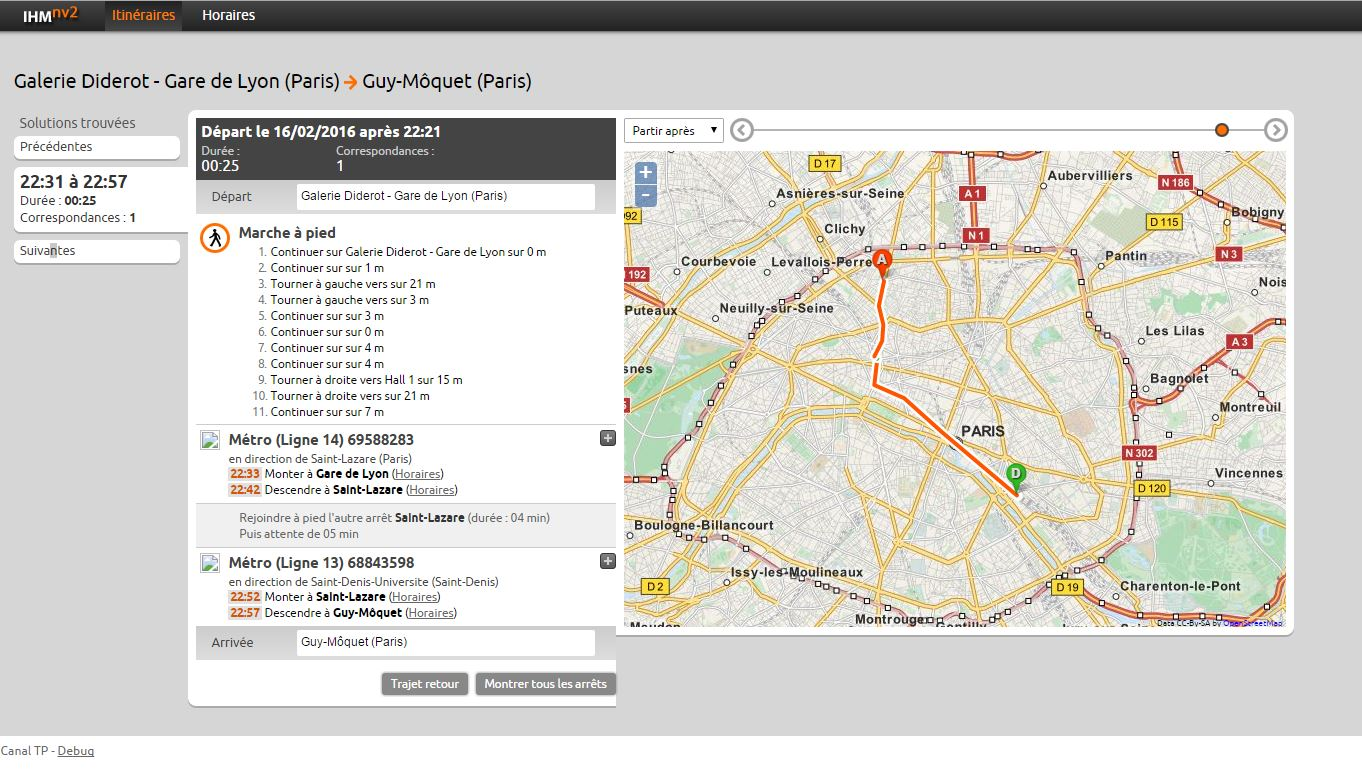
\includegraphics[height=0.22\textheight]{images/demo_navitia_io}
           \end{center}
        \item Navitia Explorer
           \begin{center}
             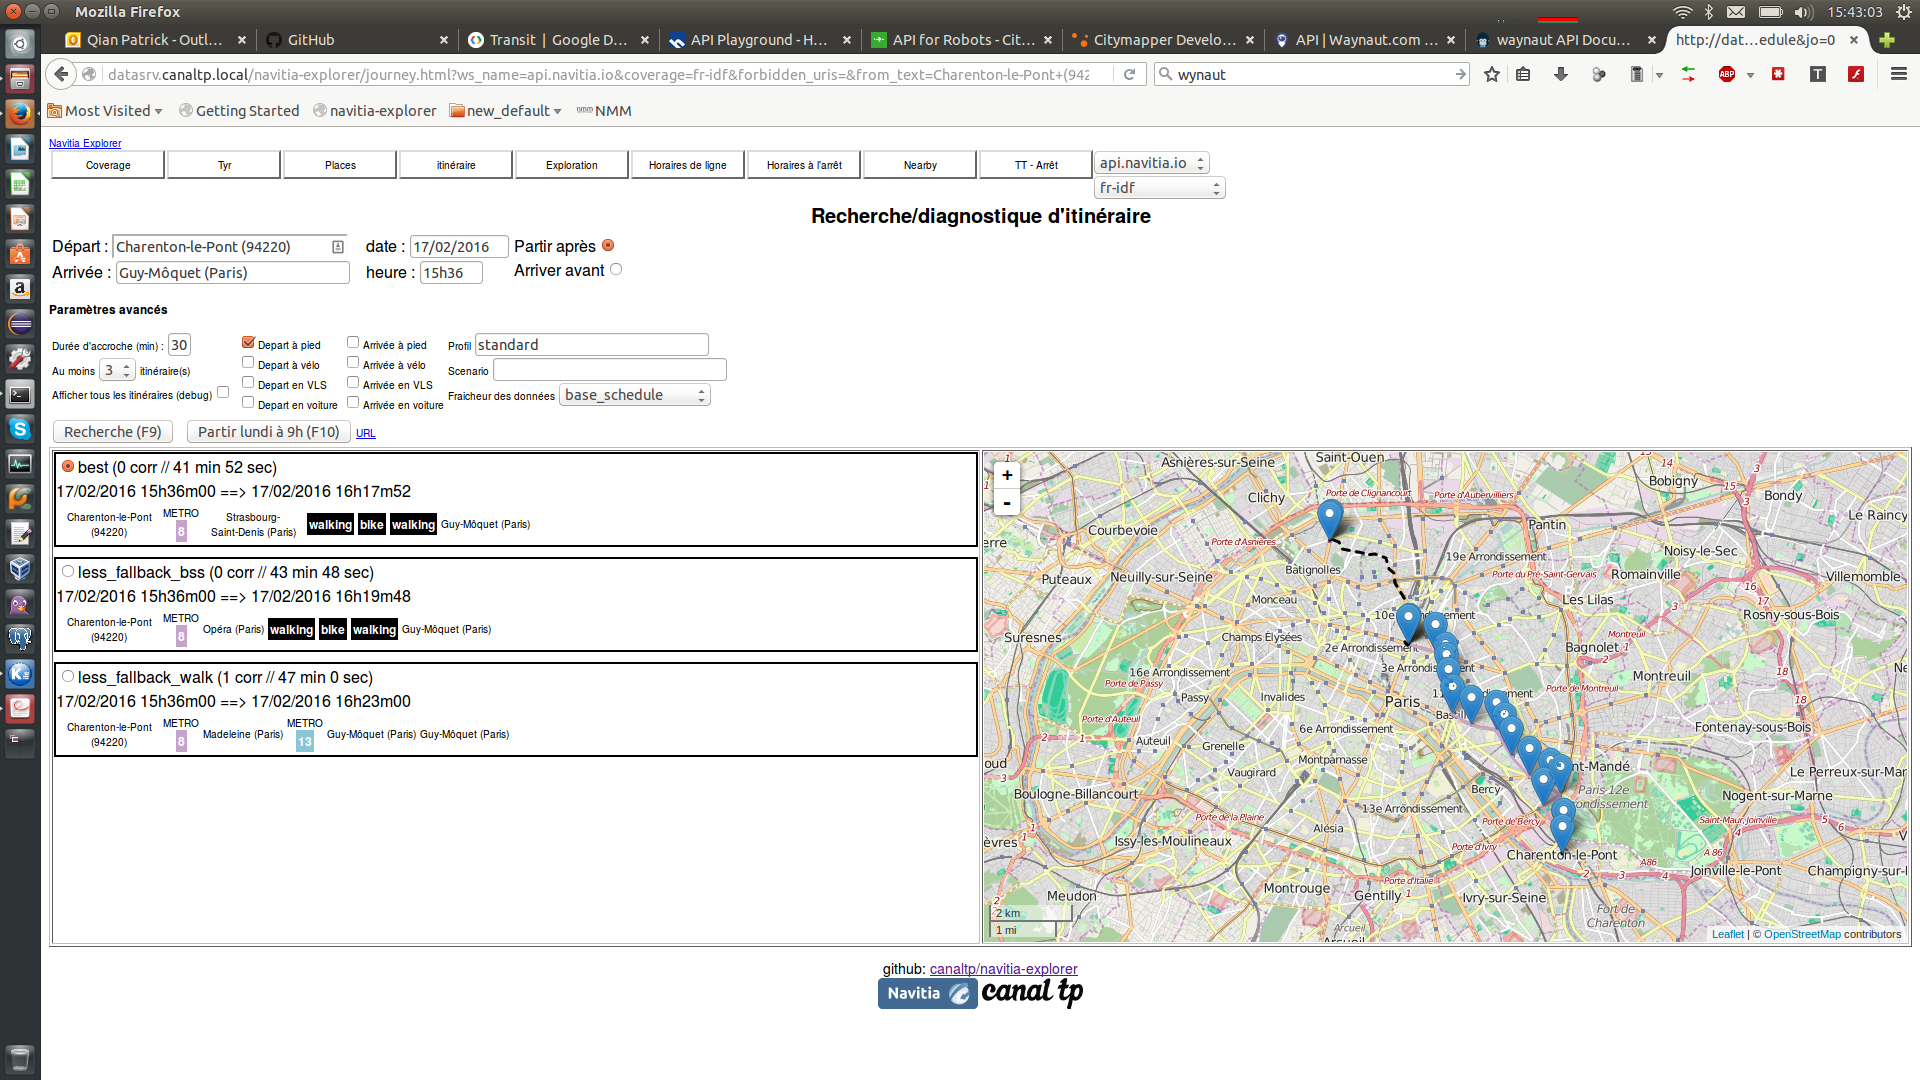
\includegraphics[height=0.22\textheight]{images/navitia-explorer}
           \end{center}
        \item IHM Artemis
          \begin{center}
            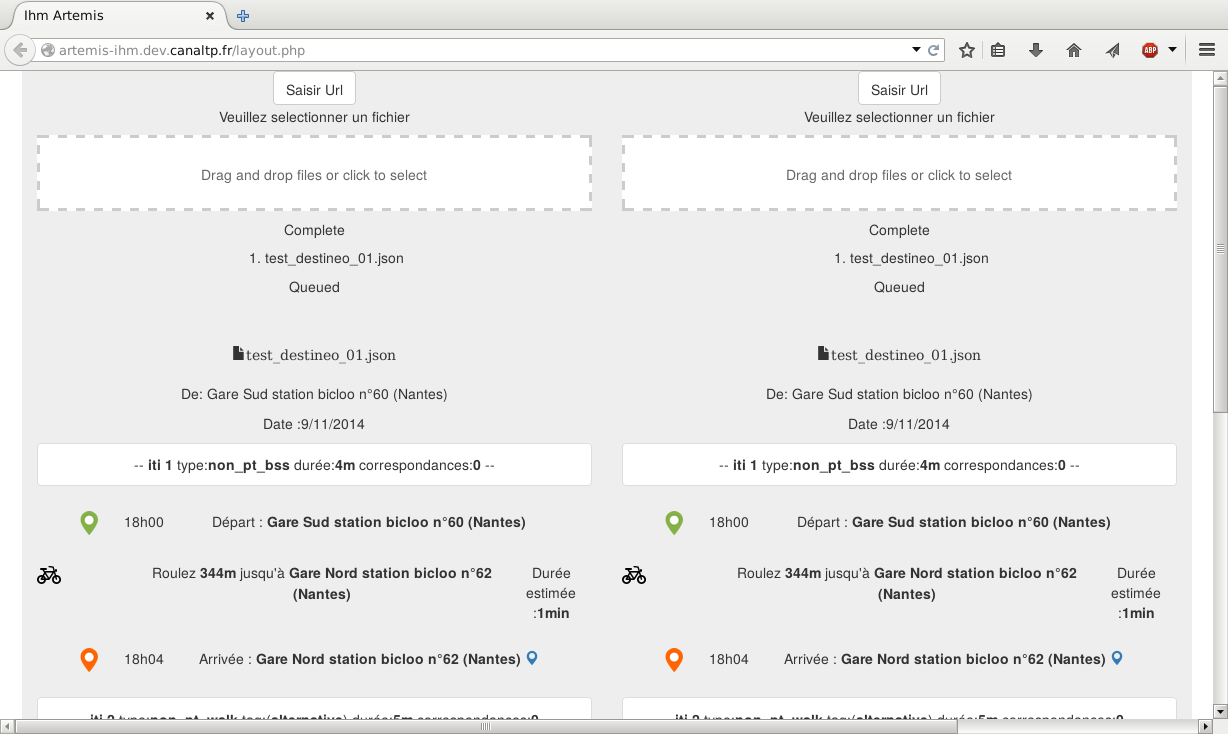
\includegraphics[height=0.24\textheight]{images/ihm-artemis}
          \end{center}
      \end{itemize}
  \end{description}
\end{frame}

\begin{frame}
  \frametitle{Solutions concurrentes internes/externes}
  \begin{description}
    \item[Externe] 
    \begin{itemize} 
      \item Swagger 
      \begin{center}
        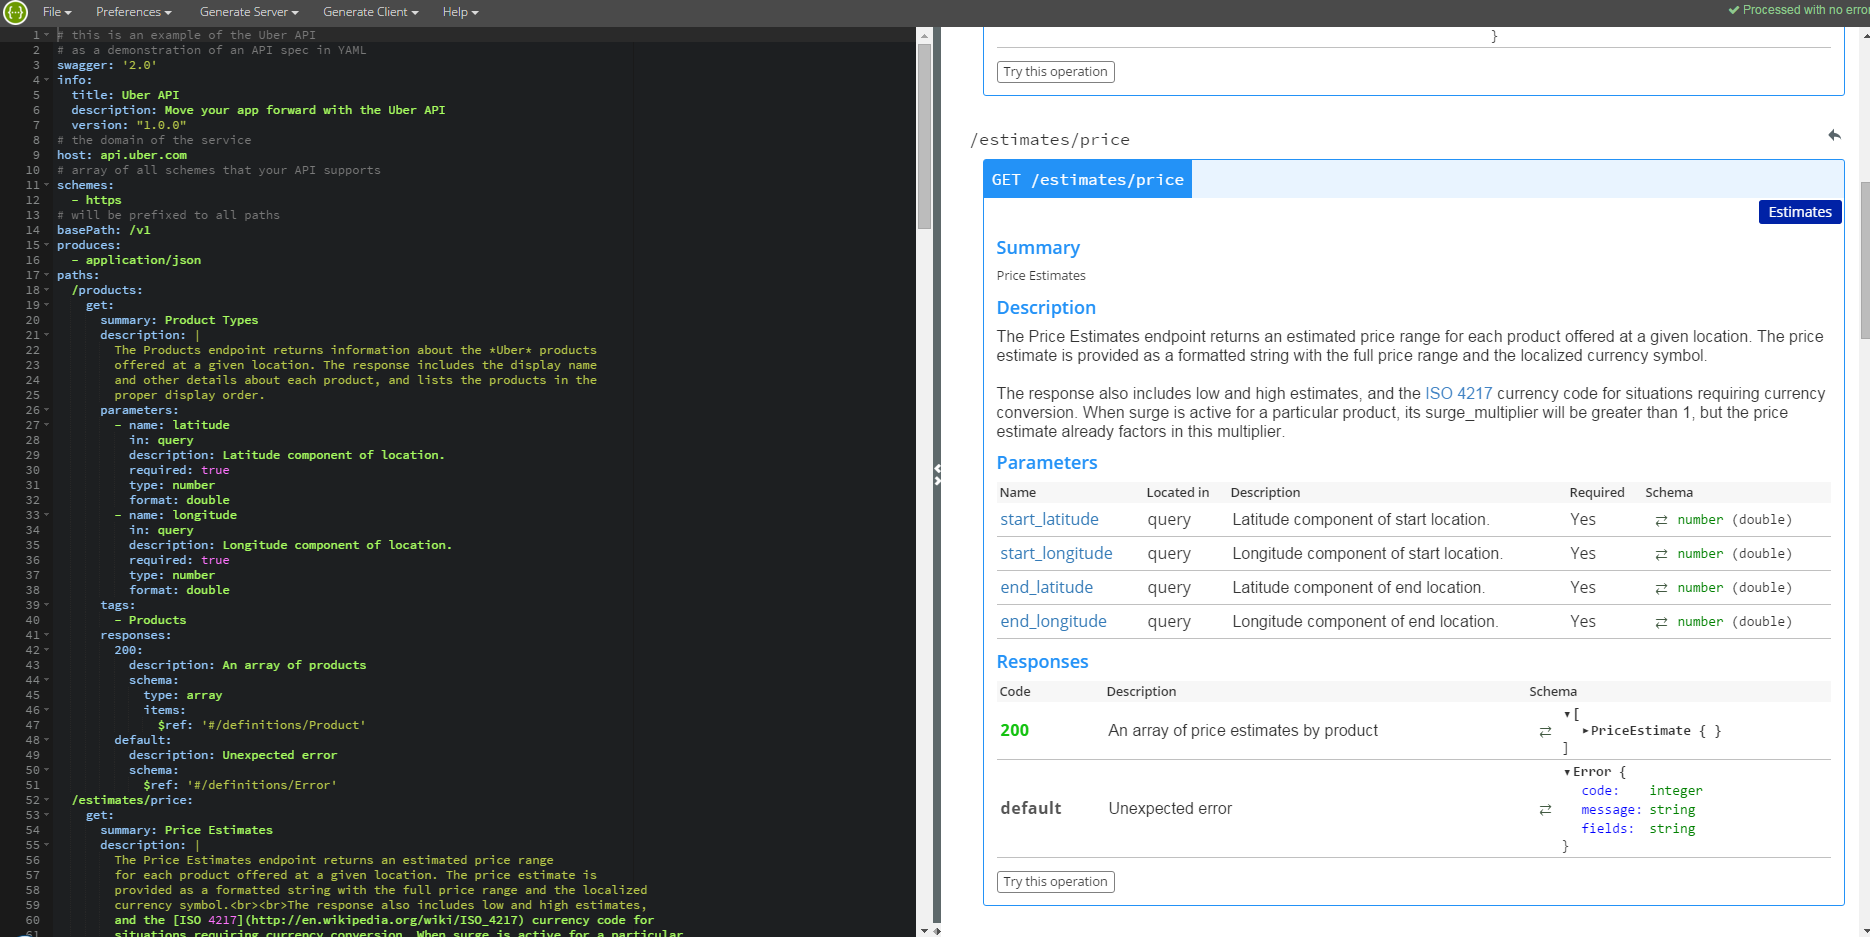
\includegraphics[height=0.3\textheight]{images/swagger}
      \end{center}
      \item MarketPlace 
      \begin{center}
        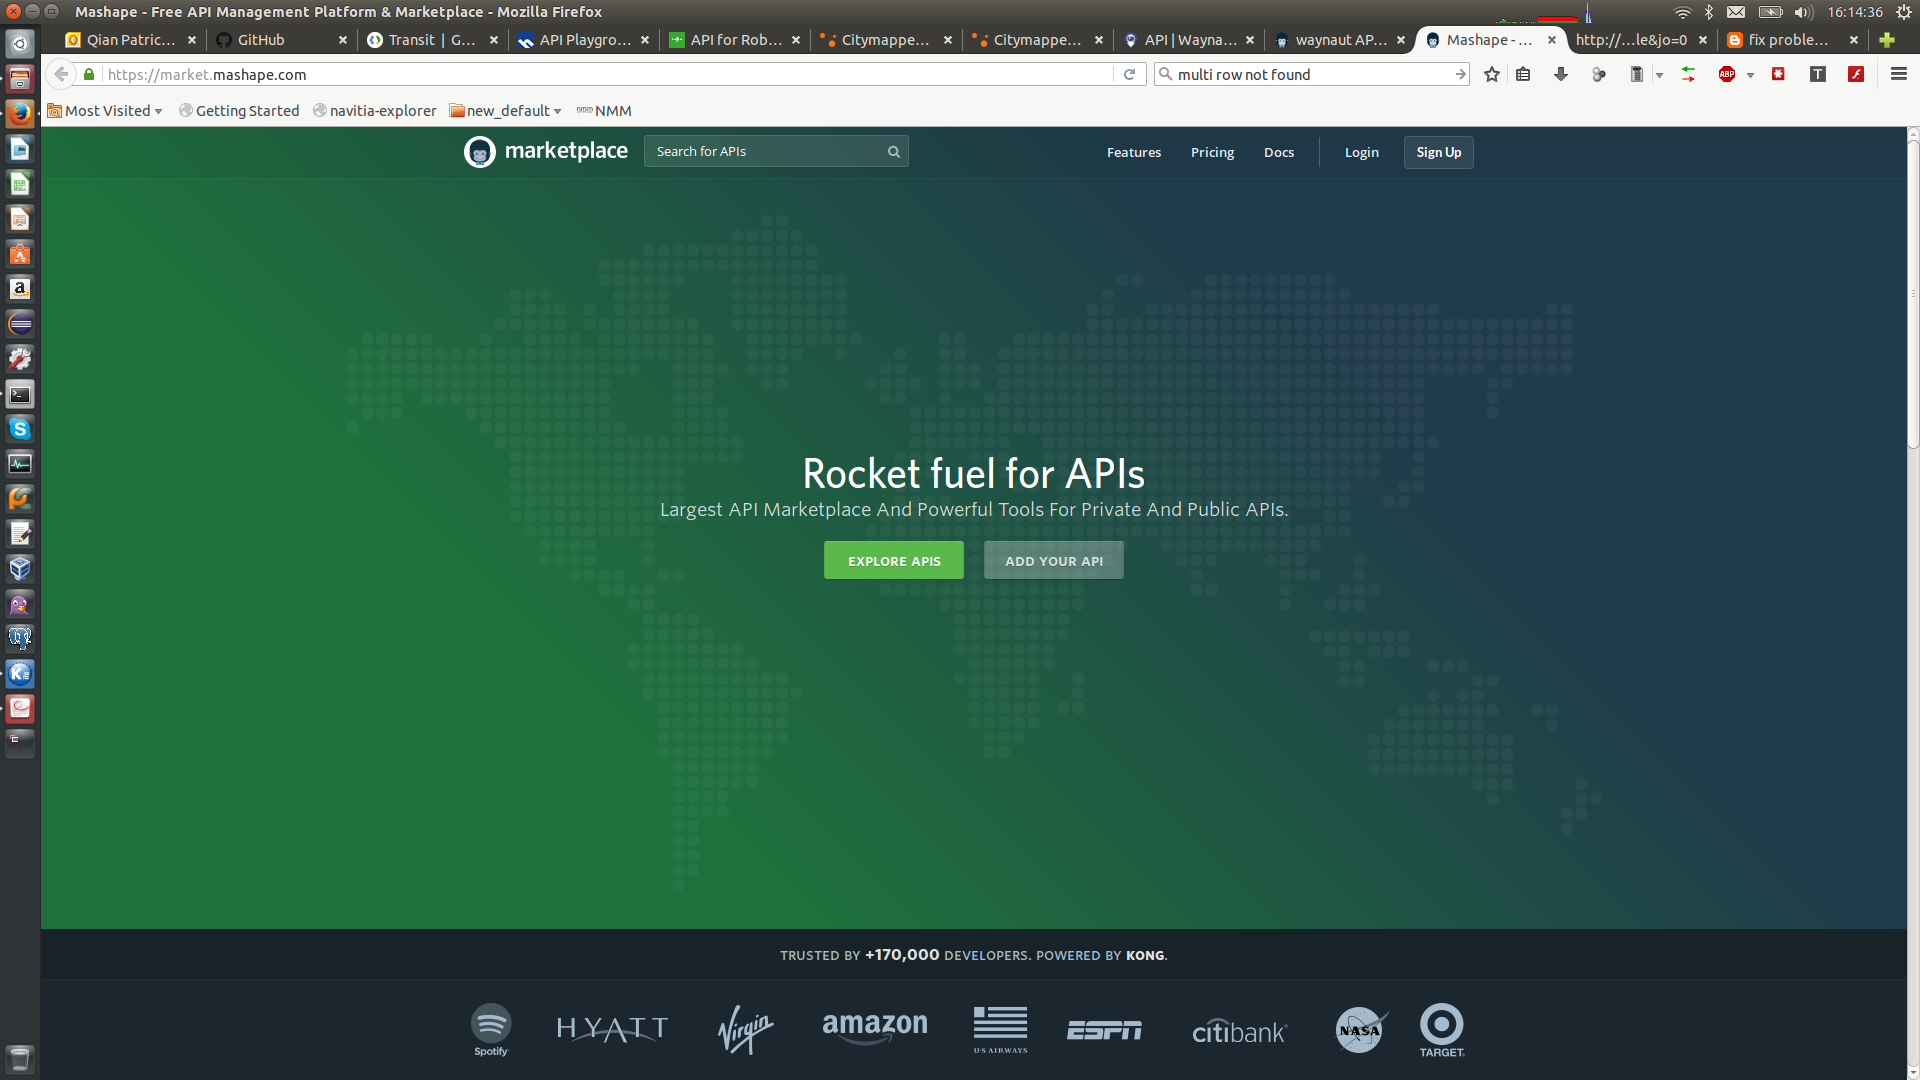
\includegraphics[height=0.3\textheight]{images/marketplace}
      \end{center}
      \item Plugin Json Firefox
      \item Json Viewer
      \item ...
    \end{itemize}
  \end{description}
\end{frame}

\begin{frame}
  \frametitle{Contexte marché dynamique}
  \begin{description}
    \item[Acteurs historiques : ]
  \end{description}
  \begin{itemize}
    \item Google Transit: Documentation
    \begin{center}
      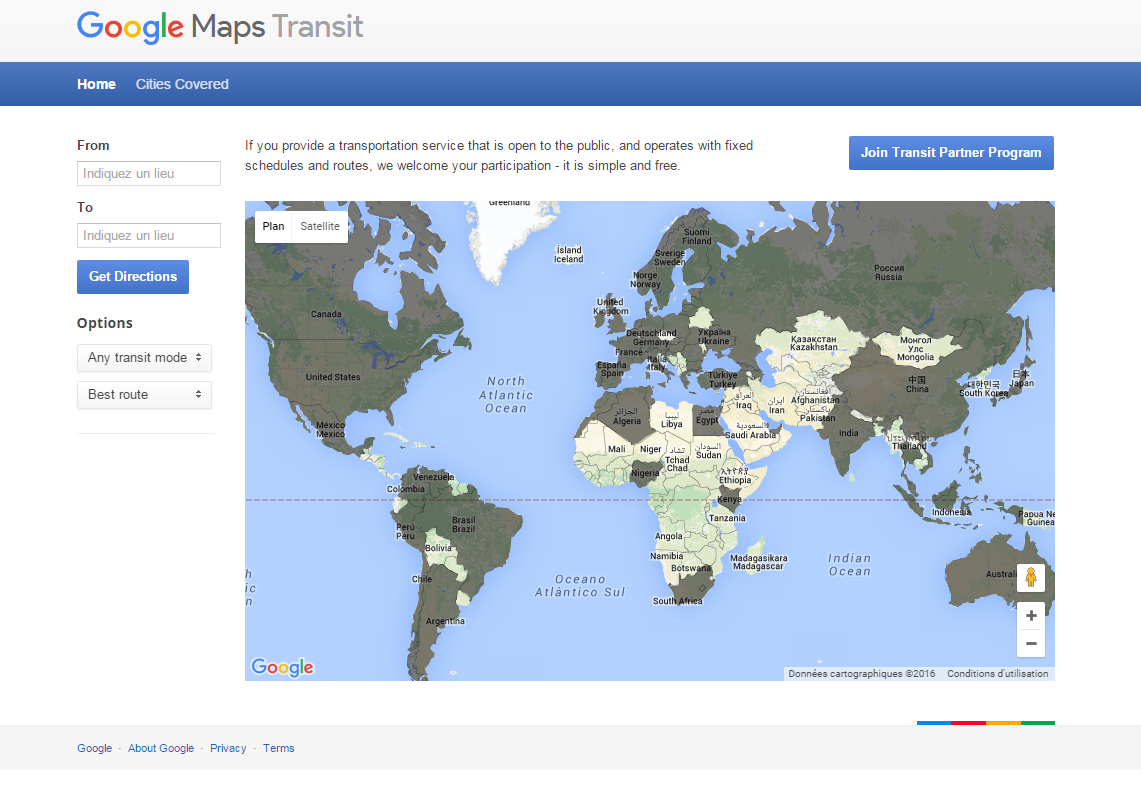
\includegraphics[height=0.4\textheight]{images/google_transit}
    \end{center}
    \item Nokia Here Transit: RESTFUL/JS API Explorer
    \begin{center}
      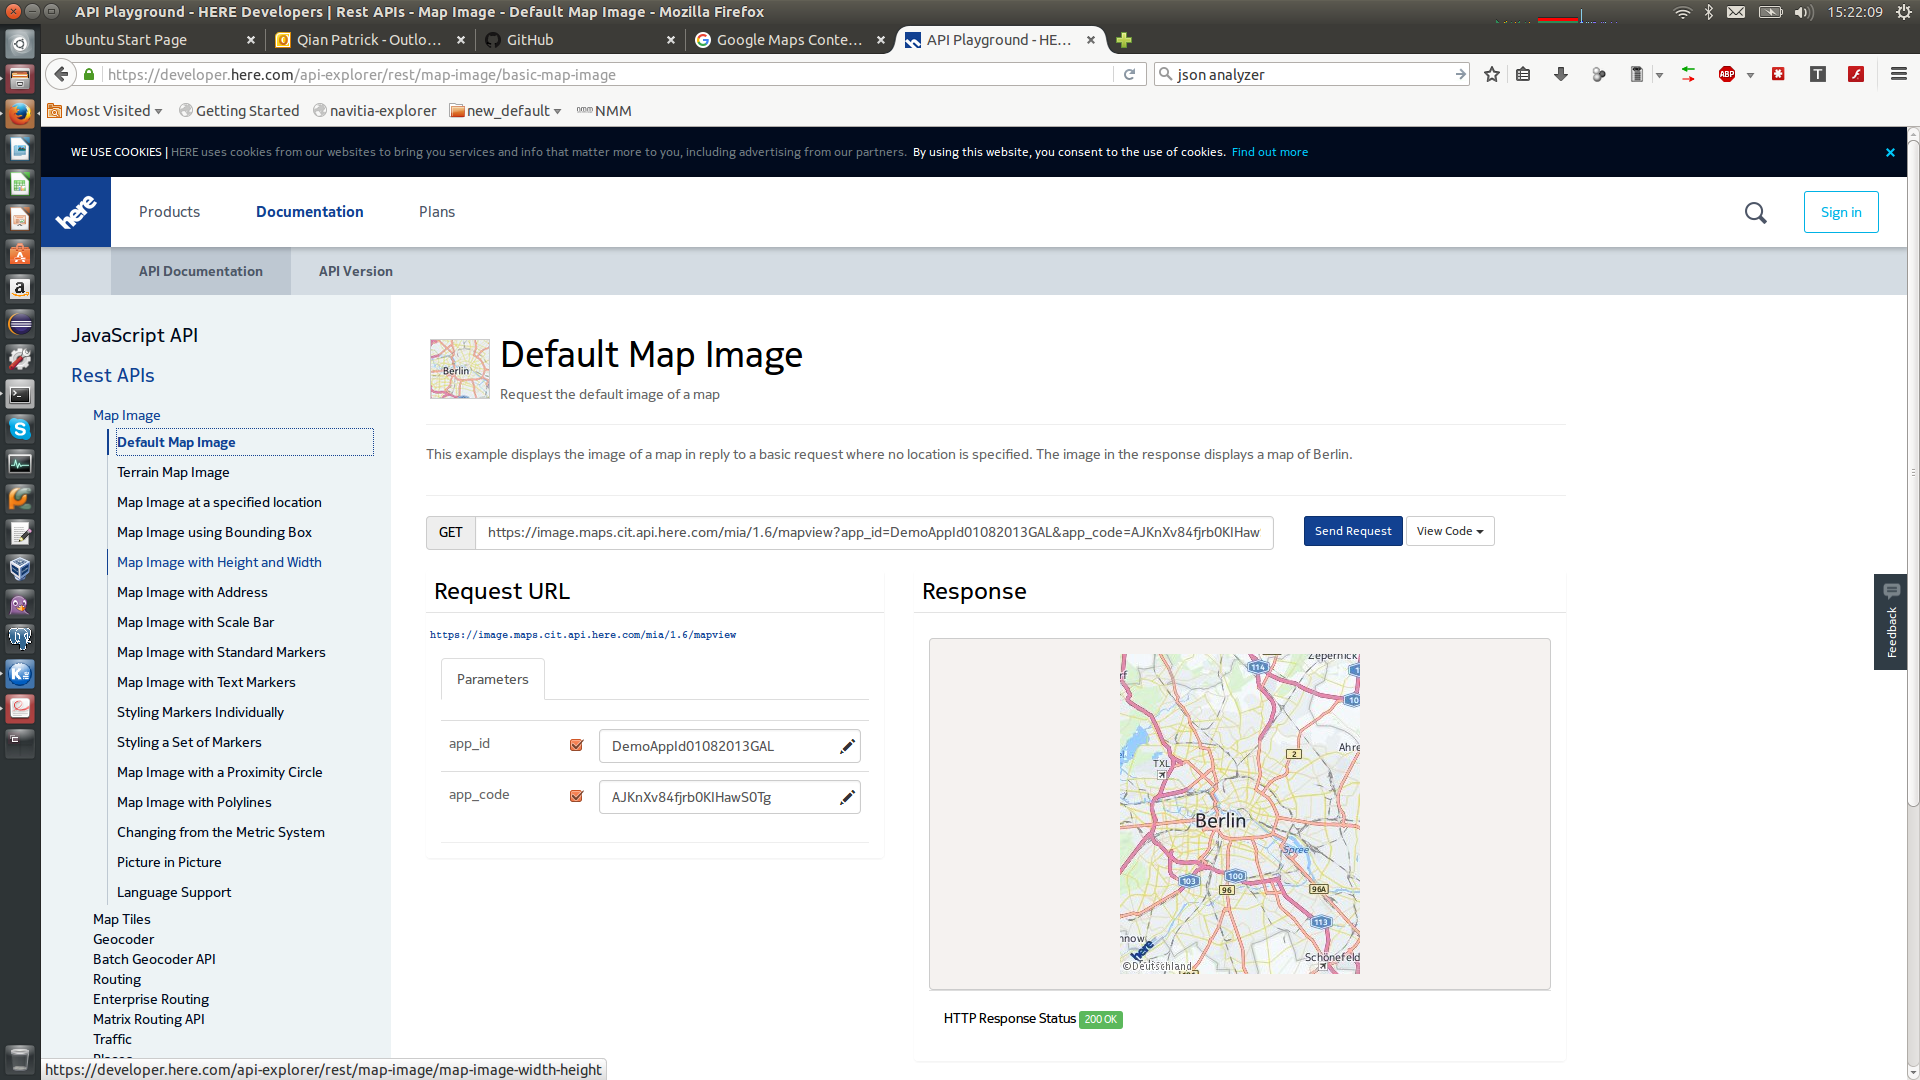
\includegraphics[height=0.25\textheight]{images/Here-API-Explorer}
    \end{center}
    
  \end{itemize}
\end{frame}

\begin{frame}
  \frametitle{Contexte marché dynamique}
  \begin{description}
    \item[Acteurs transit centric : ]
  \end{description}
  \begin{itemize}
    \item Citymapper : API et Widgets 
    \item Waynaut  :  API et Widgets (marketplace)
    \begin{center}
      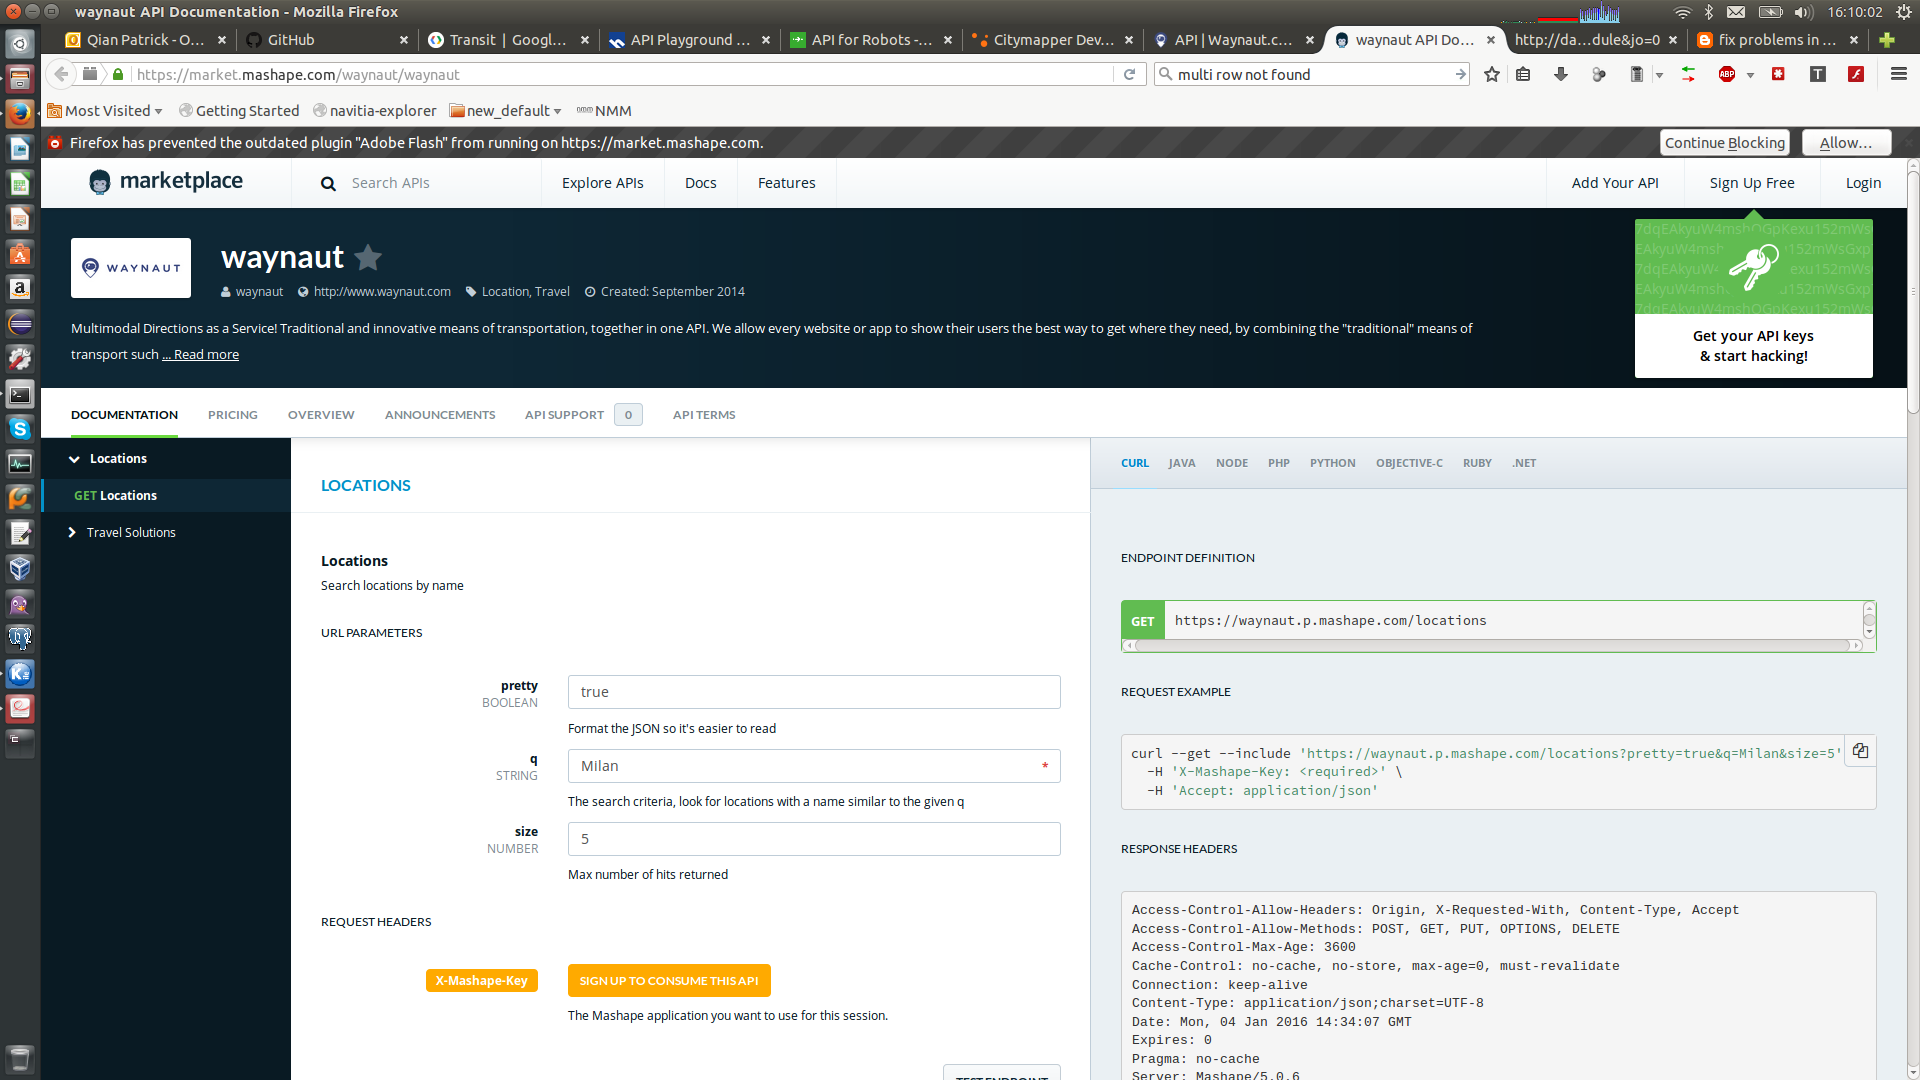
\includegraphics[height=0.25\textheight]{images/Waynaut}
    \end{center}  
    \item Transport Api : API seulement
  \end{itemize}
  \begin{description}
    \item[Acteurs open source : ]
  \end{description}
  \begin{itemize}
    \item OpenTripPlanner
  \end{itemize}
\end{frame}

\begin{frame}
  \frametitle{Audience}

  Tous les utilisateurs de navitia:
  \begin{itemize}
  \item Intégrateurs externes (développeurs, startup, SSII et pure
    players web).
  \item En interne:
    \begin{itemize}
    \item Équipes techniques (intégrateurs internes, data, RO);
    \item Support;
    \item Commercial.
    \end{itemize}
  \end{itemize}
\end{frame}

\section{Proposition de valeur}

\begin{frame}
  \frametitle{Améliorer la productivité des collaborateurs dans
    l'intégartion et le débogage de navitia}

  \centering Gains de temps en interne sur l'utilisation de navitia
  grâce à APiHM
  \vfill
  \begin{tabular}{|c|c|c|c|c|}
    \hline
    \multirow{2}{*}{Équipe}& \multicolumn{2}{c|}{par
      semaine}&nombre de&\multirow{2}{*}{Gain\footnote{1j = 7h,
        1 an = 40 semaines, 200j/an = 1 ETP}}\\
    \hhline{~--~~}
    & Avant & Après & personnes &\\
    \hline
    Data       &15h &10h & 6 & 171j/an\\
    Support    & 3h & 1h & 6 &  69j/an\\
    RO         & 2h & 1h & 8 &  46j/an\\
    NMP Mobile & 3h &1h30& 4 &  34j/an\\
    NMP Web    & 1h &40min&6 &  11j/an\\
    Q\&A       & 2h &2h30& 2 &   6j/an\\
    \hline
    \multicolumn{4}{|r|}{Total} &
    337j/an = 1{,}7 ETP\\
    \hline
  \end{tabular}
\end{frame}

\begin{frame}
  \frametitle{Outillage pour la force de vente}

  TODO: citation de Dorian

  la principale difficulté pour la force de vente consiste à
  expliciter simplement ce que permet de faire l'API à un public non
  technophile. Un outil de visualisation apporterait un atout fort
  pour accompagner leur discours et conquéruir de nouveaux clients.
\end{frame}

\begin{frame}
  \frametitle{Avantage concurrentiel}

  TODO

  Proposer des services différenciants de la concurrence, aujourd'hui
  aucun concurrents directs ne proposent des outils d'aide à la
  compréhension ou au prototypage aussi abouti que le projet APiHM.
\end{frame}

\section{Business model}

\begin{frame}
  \frametitle{Business model}

  TODO

  contexte eco de navitia.io
\end{frame}

\section{Organisation}

\begin{frame}
  \frametitle{Roadmap}

  TODO image

  3 features (question, réponse, navigation) en parallèle avec cycle:
  \begin{itemize}
  \item prototypage;
  \item tests sur utilisateurs;
  \item analyse des retours;
  \item prototypage...
  \end{itemize}

  Besoins matériels: des ordis, connexion internet, coach
  développement web front.
\end{frame}

\begin{frame}
  \frametitle{L'après SWAT}

  TODO

  Intégration navitia.io, objectif 3
\end{frame}

\section{Conclusion}

\begin{frame}
  \frametitle{Conclusion}

  TODO
\end{frame}

\begin{frame}
  \titlepage
\end{frame}

\end{document}
